% ------------------------------------------------------------------------------
% TYPO3 Version 9.3 - What's New - Chapter "Introduction" (German Version)
%
% @author	Michael Schams <schams.net>
% @license	Creative Commons BY-NC-SA 3.0
% @link		http://typo3.org/download/release-notes/whats-new/
% @language	German
% ------------------------------------------------------------------------------
% LTXE-CHAPTER-UID:		7fdf26cc-362160ab-d6c8b905-19722b20
% LTXE-CHAPTER-NAME:	Introduction
% ------------------------------------------------------------------------------

\section{Einführung}
\begin{frame}[fragile]
	\frametitle{Einführung}

	\begin{center}\huge{Einführung}\end{center}
	\begin{center}\huge{\color{typo3darkgrey}\textbf{Fakten}}\end{center}

\end{frame}

% ------------------------------------------------------------------------------
% LTXE-SLIDE-START
% LTXE-SLIDE-UID:		cbbc2090-fbe5a28c-d28df798-af2a0eea
% LTXE-SLIDE-TITLE:		TYPO3 Version 9.3 - The Facts
% ------------------------------------------------------------------------------
\begin{frame}[fragile]
	\frametitle{Einführung}
	\framesubtitle{TYPO3 Version 9.3 - Die Fakten}

	\begin{itemize}
		\item Veröffentlichungsdatum: 12 Juni 2018
		\item Releasetyp: Sprint Release
	\end{itemize}

	\begin{figure}
		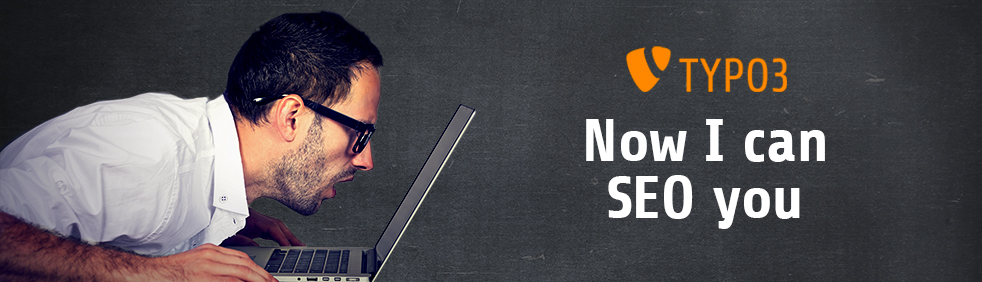
\includegraphics[width=0.95\linewidth]{Introduction/typo3-v93-banner.jpg}
	\end{figure}

\end{frame}

% ------------------------------------------------------------------------------
% LTXE-SLIDE-START
% LTXE-SLIDE-UID:		dff23213-85d734b4-8d95933a-5e45871d
% LTXE-SLIDE-TITLE:		System Requirements
% ------------------------------------------------------------------------------
\begin{frame}[fragile]
	\frametitle{Einführung}
	\framesubtitle{Systemvoraussetzungen}

	\begin{itemize}
		\item PHP version 7.2\newline
			\smaller
				(wird möglicherweise für zukünftige Versionen auf PHP 7.1 oder 7.0 herabgesetzt)
			\normalsize

		\item PHP Einstellungen:

			\begin{itemize}
				\item \texttt{memory\_limit} >= 128M
				\item \texttt{max\_execution\_time} >= 240s
				\item \texttt{max\_input\_vars} >= 1500
				\item Option \texttt{-}\texttt{-disable-ipv6} darf \underline{nicht} gesetzt sein
			\end{itemize}

		\item Die meisten von \textbf{Doctrine DBAL} unterstützten Datenbankserver arbeiten auch mit TYPO3.
			Getestete DB-Engines sind zum Beispiel:
	\end{itemize}

	\begin{figure}
		
\includegraphics[width=0.70\linewidth]{Introduction/logo-databases.png}
	\end{figure}

\end{frame}

% ------------------------------------------------------------------------------
% LTXE-SLIDE-START
% LTXE-SLIDE-UID:		f7493b39-395b22ae-44707338-fc5d2c3c
% LTXE-SLIDE-TITLE:		Development, Release and Maintenance Timeline
% ------------------------------------------------------------------------------
\begin{frame}[fragile]
	\frametitle{Einführung}
	\framesubtitle{Entwicklung, Veröffentlichung und Instandhaltung}

	\textbf{TYPO3 v9}

	\begin{figure}
		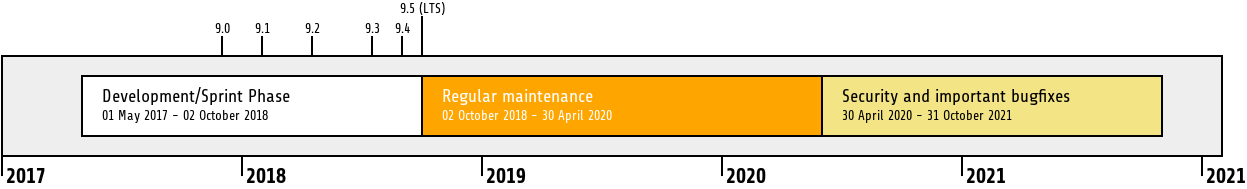
\includegraphics[width=1\linewidth]{Introduction/typo3-v9-lifecycle.png}
	\end{figure}

	\textbf{Erweiterter Support}\newline
	\smaller
		Die \href{https://typo3.com}{TYPO3 GmbH} bietet weitere Supportmöglichkeiten
		für TYPO3 v9 LTS auch nach dem 31. Oktober 2021 für bis zu zwei weitere Jahre.
	\normalsize

%	\url{https://typo3.com/our-services/extended-support/}

\end{frame}

% ------------------------------------------------------------------------------
% LTXE-SLIDE-START
% LTXE-SLIDE-UID:		401dc930-4fe56f55-b9f30577-2b8c7f7d
% LTXE-SLIDE-TITLE:		TYPO3 v9 Roadmap
% ------------------------------------------------------------------------------
\begin{frame}[fragile]
	\frametitle{Einführung}
	\framesubtitle{TYPO3 v9 Roadmap}

	Voraussichtliche Veröffentlichungen und deren Hauptfokus:

	\begin{itemize}

		\item v9.0 \tabto{1.1cm}12/Dez/2017\tabto{3.4cm}Install Tool and Page Tree Refactoring,\newline
			\tabto{3.4cm}Unified Page Translations
		\item v9.1 \tabto{1.1cm}30/Jan/2018\tabto{3.4cm}Redirect Handling
		\item v9.2 \tabto{1.1cm}10/Apr/2018\tabto{3.4cm}Site Handling
		\item
			\begingroup
				\color{typo3orange}
					v9.3 \tabto{1.1cm}12/Jun/2018\tabto{3.4cm}SEO and URL Routing Preparations
			\endgroup
		\item v9.4 \tabto{1.1cm}04/Sep/2018\tabto{3.4cm}Frontend Editing (Feature Freeze)
		\item v9.5 \tabto{1.1cm}02/Okt/2018\tabto{3.4cm}LTS Release

	\end{itemize}

	\smaller
		\url{https://typo3.org/news/article/typo3-v9-roadmap/}\newline
		\url{https://typo3.org/typo3-cms/roadmap/}
	\normalsize

\end{frame}

% ------------------------------------------------------------------------------
% LTXE-SLIDE-START
% LTXE-SLIDE-UID:		9d7a8e4c-8ce3a51b-a55f5371-2b8998a7
% LTXE-SLIDE-TITLE:		Installation
% ------------------------------------------------------------------------------
\begin{frame}[fragile]
	\frametitle{Einführung}
	\framesubtitle{Installation}

	\begin{itemize}
		\item Empfohlene \textit{klassische} Installationsschritte unter Linux/Mac OS X\newline
			(DocumentRoot ist beispielsweise \texttt{/var/www/site/htdocs}):
		\begin{lstlisting}
			$ cd /var/www/site
			$ wget --content-disposition get.typo3.org/9.3
			$ tar xzf typo3_src-9.3.0.tar.gz
			$ cd htdocs
			$ ln -s ../typo3_src-9.3.0 typo3_src
			$ ln -s typo3_src/index.php
			$ ln -s typo3_src/typo3
			$ touch FIRST_INSTALL
		\end{lstlisting}

		\item Symbolische Links unter Microsoft Windows:

			\begin{itemize}
				\item unter Windows XP/2000 kann \texttt{junction} benutzt werden
				\item unter Windows Vista und Windows 7 oder höher kann \texttt{mklink} benutzt werden
			\end{itemize}

	\end{itemize}
\end{frame}

% ------------------------------------------------------------------------------
% LTXE-SLIDE-START
% LTXE-SLIDE-UID:		3334275d-634795ed-90079c68-83d70096
% LTXE-SLIDE-TITLE:		Installation using composer
% ------------------------------------------------------------------------------
\begin{frame}[fragile]
	\frametitle{Installation}
	\framesubtitle{Installation mit \texttt{composer}}

	% decrease font size for code listing
	\lstset{basicstyle=\tiny\ttfamily}

	\begin{itemize}
		\item Installation mit \textit{composer} unter Linux, Mac OS X und Windows 10:

			\begin{lstlisting}
				$ cd /var/www/site/
				$ composer create-project typo3/cms-base-distribution CmsBaseDistribution ^9
			\end{lstlisting}

		\item Alternativ kann man eine benutzerdefinierte \texttt{composer.json} Datei erstellen und ausführen:

			\begin{lstlisting}
				$ composer install
			\end{lstlisting}

			Weitere \texttt{composer.json} Beispielsdateien können unter \href{https://composer.typo3.org}{https://composer.typo3.org} heruntergeladen werden
			\normalsize

	\end{itemize}
\end{frame}

% ------------------------------------------------------------------------------
